\documentclass[12pt]{article}
\usepackage{graphicx}
\usepackage{ragged2e}
\usepackage{array}
\newcolumntype{L}[1]{>{\raggedright\let\newline\\\arraybackslash\hspace{0pt}}m{#1}}
\newcolumntype{C}[1]{>{\centering\let\newline\\\arraybackslash\hspace{0pt}}m{#1}}
\newcolumntype{R}[1]{>{\raggedleft\let\newline\\\arraybackslash\hspace{0pt}}m{#1}}

\begin{document}
	\centering{\bf{KOLHAPUR INSTITUTE OF TECHNOLOGY'S}}\par
	{\bf{COLLEGE OF ENGINEERING (AUTONOMOUS),KOLHAPUR}}
	\par\noindent\rule{\textwidth}{0.4pt}
	
	\centering{\bf{First Year BTech}}\par
	\centering{\bf{MID SEMESTER EXAMINATION}}\par
	\centering{\bf{Web Technologies (wt1)}}\par
\begin{flushleft}
	Day and Date :{}\hspace{5.5cm}PRN:
\end{flushleft}

\begin{flushleft}
	Time :{}\hspace{7cm}Max Marks:{50}\\
\end{flushleft}
\noindent\rule{\textwidth}{0.1pt}
\begin{flushleft}
	{\bf Instructions:}\\
	{\hspace{0.5cm} \bf IMP: Verify that you have received question paper with correct course, code, branch, etc}\\
	\hspace{1cm}i) All Questions are Compulsory\\
	\hspace{1cm}ii)Figure to right indicate full marks\\
	\hspace{1cm}iii)Assume suitable data wherever necessary\\
\end{flushleft} 

	\begin{flushleft}
	\bf{QNo}\hspace{1.2cm} \bf{Question} \hspace{5.5cm}  \bf{Marks} \hspace{0.2cm} \bf{CO} \hspace{0.2cm}	\bf{BL}	
	
	
	
	
	
	
\end{flushleft}

		

	
	
	\begin{tabular}{|L{1cm}|L{8cm}|C{1cm}|C{1cm}|C{1cm}|}\hline
			\bf1 & \bf{Attempt} \bf1 out of \bf2 & \bf16 & & \\ \hline
				1.A &
	Image1 Question again \newline
		\begin{center}
		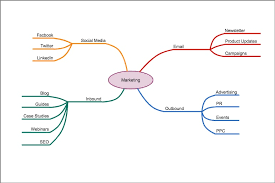
\includegraphics[width=4cm,height=3cm]{media/diagrams/image1.png}\\\bf{Figure }\bf1.A	
	\end{center}

	
		 &  1 & CO1 & 1\\ \hline
		1.B &
	what is javascript? \newline
		 &  1 & CO1 & 1\\ \hline
		\end{tabular}

	
	


	
	
		

	
	
	\begin{tabular}{|L{1cm}|L{8cm}|C{1cm}|C{1cm}|C{1cm}|}\hline
			\bf2 & \bf{Attempt} \bf1 out of \bf2 & \bf16 & & \\ \hline
				2.A &
	Image1 Question \newline
		 &  1 & CO1 & 1\\ \hline
		2.B &
	image3 question \newline
		\begin{center}
		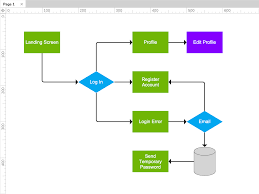
\includegraphics[width=4cm,height=3cm]{media/diagrams/image3.png}\\\bf{Figure }\bf2.B	
	\end{center}

	
		 &  1 & CO4 & 1\\ \hline
		\end{tabular}

	
	


	
	
		

	
	
	\begin{tabular}{|L{1cm}|L{8cm}|C{1cm}|C{1cm}|C{1cm}|}\hline
			\bf3 & \bf{Attempt} \bf1 out of \bf2 & \bf16 & & \\ \hline
				3.A &
	Explain with characteristics the React.js Framework. \newline
		 &  1 & CO1 & 1\\ \hline
		3.B &
	 \newline
		 &   & CO & \\ \hline
		\end{tabular}

	
	


	
	
		
	
\end{document}